\documentclass[]{article}
\usepackage{lmodern}
\usepackage{amssymb,amsmath}
\usepackage{ifxetex,ifluatex}
\usepackage{fixltx2e} % provides \textsubscript
\ifnum 0\ifxetex 1\fi\ifluatex 1\fi=0 % if pdftex
  \usepackage[T1]{fontenc}
  \usepackage[utf8]{inputenc}
\else % if luatex or xelatex
  \ifxetex
    \usepackage{mathspec}
  \else
    \usepackage{fontspec}
  \fi
  \defaultfontfeatures{Ligatures=TeX,Scale=MatchLowercase}
\fi
% use upquote if available, for straight quotes in verbatim environments
\IfFileExists{upquote.sty}{\usepackage{upquote}}{}
% use microtype if available
\IfFileExists{microtype.sty}{%
\usepackage{microtype}
\UseMicrotypeSet[protrusion]{basicmath} % disable protrusion for tt fonts
}{}
\usepackage[margin=1in]{geometry}
\usepackage{hyperref}
\hypersetup{unicode=true,
            pdftitle={Bioinformatics Class 7},
            pdfauthor={Andrew Valadez},
            pdfborder={0 0 0},
            breaklinks=true}
\urlstyle{same}  % don't use monospace font for urls
\usepackage{color}
\usepackage{fancyvrb}
\newcommand{\VerbBar}{|}
\newcommand{\VERB}{\Verb[commandchars=\\\{\}]}
\DefineVerbatimEnvironment{Highlighting}{Verbatim}{commandchars=\\\{\}}
% Add ',fontsize=\small' for more characters per line
\usepackage{framed}
\definecolor{shadecolor}{RGB}{248,248,248}
\newenvironment{Shaded}{\begin{snugshade}}{\end{snugshade}}
\newcommand{\KeywordTok}[1]{\textcolor[rgb]{0.13,0.29,0.53}{\textbf{#1}}}
\newcommand{\DataTypeTok}[1]{\textcolor[rgb]{0.13,0.29,0.53}{#1}}
\newcommand{\DecValTok}[1]{\textcolor[rgb]{0.00,0.00,0.81}{#1}}
\newcommand{\BaseNTok}[1]{\textcolor[rgb]{0.00,0.00,0.81}{#1}}
\newcommand{\FloatTok}[1]{\textcolor[rgb]{0.00,0.00,0.81}{#1}}
\newcommand{\ConstantTok}[1]{\textcolor[rgb]{0.00,0.00,0.00}{#1}}
\newcommand{\CharTok}[1]{\textcolor[rgb]{0.31,0.60,0.02}{#1}}
\newcommand{\SpecialCharTok}[1]{\textcolor[rgb]{0.00,0.00,0.00}{#1}}
\newcommand{\StringTok}[1]{\textcolor[rgb]{0.31,0.60,0.02}{#1}}
\newcommand{\VerbatimStringTok}[1]{\textcolor[rgb]{0.31,0.60,0.02}{#1}}
\newcommand{\SpecialStringTok}[1]{\textcolor[rgb]{0.31,0.60,0.02}{#1}}
\newcommand{\ImportTok}[1]{#1}
\newcommand{\CommentTok}[1]{\textcolor[rgb]{0.56,0.35,0.01}{\textit{#1}}}
\newcommand{\DocumentationTok}[1]{\textcolor[rgb]{0.56,0.35,0.01}{\textbf{\textit{#1}}}}
\newcommand{\AnnotationTok}[1]{\textcolor[rgb]{0.56,0.35,0.01}{\textbf{\textit{#1}}}}
\newcommand{\CommentVarTok}[1]{\textcolor[rgb]{0.56,0.35,0.01}{\textbf{\textit{#1}}}}
\newcommand{\OtherTok}[1]{\textcolor[rgb]{0.56,0.35,0.01}{#1}}
\newcommand{\FunctionTok}[1]{\textcolor[rgb]{0.00,0.00,0.00}{#1}}
\newcommand{\VariableTok}[1]{\textcolor[rgb]{0.00,0.00,0.00}{#1}}
\newcommand{\ControlFlowTok}[1]{\textcolor[rgb]{0.13,0.29,0.53}{\textbf{#1}}}
\newcommand{\OperatorTok}[1]{\textcolor[rgb]{0.81,0.36,0.00}{\textbf{#1}}}
\newcommand{\BuiltInTok}[1]{#1}
\newcommand{\ExtensionTok}[1]{#1}
\newcommand{\PreprocessorTok}[1]{\textcolor[rgb]{0.56,0.35,0.01}{\textit{#1}}}
\newcommand{\AttributeTok}[1]{\textcolor[rgb]{0.77,0.63,0.00}{#1}}
\newcommand{\RegionMarkerTok}[1]{#1}
\newcommand{\InformationTok}[1]{\textcolor[rgb]{0.56,0.35,0.01}{\textbf{\textit{#1}}}}
\newcommand{\WarningTok}[1]{\textcolor[rgb]{0.56,0.35,0.01}{\textbf{\textit{#1}}}}
\newcommand{\AlertTok}[1]{\textcolor[rgb]{0.94,0.16,0.16}{#1}}
\newcommand{\ErrorTok}[1]{\textcolor[rgb]{0.64,0.00,0.00}{\textbf{#1}}}
\newcommand{\NormalTok}[1]{#1}
\usepackage{graphicx,grffile}
\makeatletter
\def\maxwidth{\ifdim\Gin@nat@width>\linewidth\linewidth\else\Gin@nat@width\fi}
\def\maxheight{\ifdim\Gin@nat@height>\textheight\textheight\else\Gin@nat@height\fi}
\makeatother
% Scale images if necessary, so that they will not overflow the page
% margins by default, and it is still possible to overwrite the defaults
% using explicit options in \includegraphics[width, height, ...]{}
\setkeys{Gin}{width=\maxwidth,height=\maxheight,keepaspectratio}
\IfFileExists{parskip.sty}{%
\usepackage{parskip}
}{% else
\setlength{\parindent}{0pt}
\setlength{\parskip}{6pt plus 2pt minus 1pt}
}
\setlength{\emergencystretch}{3em}  % prevent overfull lines
\providecommand{\tightlist}{%
  \setlength{\itemsep}{0pt}\setlength{\parskip}{0pt}}
\setcounter{secnumdepth}{0}
% Redefines (sub)paragraphs to behave more like sections
\ifx\paragraph\undefined\else
\let\oldparagraph\paragraph
\renewcommand{\paragraph}[1]{\oldparagraph{#1}\mbox{}}
\fi
\ifx\subparagraph\undefined\else
\let\oldsubparagraph\subparagraph
\renewcommand{\subparagraph}[1]{\oldsubparagraph{#1}\mbox{}}
\fi

%%% Use protect on footnotes to avoid problems with footnotes in titles
\let\rmarkdownfootnote\footnote%
\def\footnote{\protect\rmarkdownfootnote}

%%% Change title format to be more compact
\usepackage{titling}

% Create subtitle command for use in maketitle
\newcommand{\subtitle}[1]{
  \posttitle{
    \begin{center}\large#1\end{center}
    }
}

\setlength{\droptitle}{-2em}
  \title{Bioinformatics Class 7}
  \pretitle{\vspace{\droptitle}\centering\huge}
  \posttitle{\par}
  \author{Andrew Valadez}
  \preauthor{\centering\large\emph}
  \postauthor{\par}
  \predate{\centering\large\emph}
  \postdate{\par}
  \date{April 25, 2018}


\begin{document}
\maketitle

\section{Functions again}\label{functions-again}

We can source any file of R code with the `source'() function.

alt control i gives the insert shortcut

\begin{Shaded}
\begin{Highlighting}[]
\KeywordTok{source}\NormalTok{(}\StringTok{"http://tinyurl.com/rescale-R"}\NormalTok{)}
\end{Highlighting}
\end{Shaded}

have the rescale thing and when try to open it will have spectacles and
that means it is read only function take x find range and will have an
answer

Lets make sure things are here ls will list things in envrionment

\begin{Shaded}
\begin{Highlighting}[]
\KeywordTok{ls}\NormalTok{()}
\end{Highlighting}
\end{Shaded}

\begin{verbatim}
##  [1] "both_na"         "both_na2"        "both_na3"       
##  [4] "df1"             "df2"             "df3"            
##  [7] "gene_intersect"  "gene_intersect2" "gene_intersect3"
## [10] "gene_intersect4" "rescale"         "rescale2"
\end{verbatim}

Check our rescale function is working

\begin{Shaded}
\begin{Highlighting}[]
\KeywordTok{rescale}\NormalTok{(}\DecValTok{1}\OperatorTok{:}\DecValTok{10}\NormalTok{)}
\end{Highlighting}
\end{Shaded}

\begin{verbatim}
##  [1] 0.0000000 0.1111111 0.2222222 0.3333333 0.4444444 0.5555556 0.6666667
##  [8] 0.7777778 0.8888889 1.0000000
\end{verbatim}

\begin{Shaded}
\begin{Highlighting}[]
\KeywordTok{rescale}\NormalTok{( }\KeywordTok{c}\NormalTok{(}\DecValTok{1}\OperatorTok{:}\DecValTok{10}\NormalTok{,}\StringTok{"tacobell"}\NormalTok{))}
\end{Highlighting}
\end{Shaded}

no real help out of the error message, how do we catch these kind of
things to fail ealry and fail largely?

introduce warning() and stop() warning will continue running the fx stop
will just terminate the action of the fx

lets use that approach to fail early and largely

adding rescale if function if whatever in parenthese is true then will
go through the rest of it so if true will go inside if to the stop x is
our input here the fx is numeric and has an exclamation mark

is .numeric tests to see if input is all numbers , the input in script
with the string tacobell

\begin{Shaded}
\begin{Highlighting}[]
\ControlFlowTok{function}\NormalTok{(x, }\DataTypeTok{na.rm=}\OtherTok{TRUE}\NormalTok{, }\DataTypeTok{plot=}\OtherTok{FALSE}\NormalTok{, ...) \{}
  \CommentTok{# Our rescale function from lecture 10}

  \ControlFlowTok{if}\NormalTok{( }\OperatorTok{!}\KeywordTok{is.numeric}\NormalTok{(x) ) \{}
    \KeywordTok{stop}\NormalTok{(}\StringTok{"Input x should be numeric"}\NormalTok{, }\DataTypeTok{call.=}\OtherTok{FALSE}\NormalTok{)}
\NormalTok{  \}}
  
\NormalTok{  rng <-}\KeywordTok{range}\NormalTok{(x, }\DataTypeTok{na.rm=}\OtherTok{TRUE}\NormalTok{)}

\NormalTok{  answer <-}\StringTok{ }\NormalTok{(x }\OperatorTok{-}\StringTok{ }\NormalTok{rng[}\DecValTok{1}\NormalTok{]) }\OperatorTok{/}\StringTok{ }\NormalTok{(rng[}\DecValTok{2}\NormalTok{] }\OperatorTok{-}\StringTok{ }\NormalTok{rng[}\DecValTok{1}\NormalTok{])}
  \ControlFlowTok{if}\NormalTok{(plot) \{ }
    \KeywordTok{plot}\NormalTok{(answer, ...) }
\NormalTok{  \}}

  \KeywordTok{return}\NormalTok{(answer)}
\NormalTok{\}}
\end{Highlighting}
\end{Shaded}

\begin{verbatim}
## function(x, na.rm=TRUE, plot=FALSE, ...) {
##   # Our rescale function from lecture 10
## 
##   if( !is.numeric(x) ) {
##     stop("Input x should be numeric", call.=FALSE)
##   }
##   
##   rng <-range(x, na.rm=TRUE)
## 
##   answer <- (x - rng[1]) / (rng[2] - rng[1])
##   if(plot) { 
##     plot(answer, ...) 
##   }
## 
##   return(answer)
## }
\end{verbatim}

\begin{Shaded}
\begin{Highlighting}[]
\KeywordTok{is.numeric}\NormalTok{(}\KeywordTok{c}\NormalTok{(}\DecValTok{1}\OperatorTok{:}\DecValTok{10}\NormalTok{,}\StringTok{"tacobell"}\NormalTok{))}
\end{Highlighting}
\end{Shaded}

\begin{verbatim}
## [1] FALSE
\end{verbatim}

this is false it isnt numbers in fx had exclamation mark flips it so
makes false true

\begin{Shaded}
\begin{Highlighting}[]
\OperatorTok{!}\KeywordTok{is.numeric}\NormalTok{((}\KeywordTok{c}\NormalTok{(}\DecValTok{1}\OperatorTok{:}\DecValTok{10}\NormalTok{,}\StringTok{"tacobell"}\NormalTok{)))}
\end{Highlighting}
\end{Shaded}

\begin{verbatim}
## [1] TRUE
\end{verbatim}

lets open rescale2 again call.=false is good to not overcomplicate why
it failed lets test it though rescale gave error with tacobell

\begin{Shaded}
\begin{Highlighting}[]
\ControlFlowTok{function}\NormalTok{(x, }\DataTypeTok{na.rm=}\OtherTok{TRUE}\NormalTok{, }\DataTypeTok{plot=}\OtherTok{FALSE}\NormalTok{, ...) \{}
  \CommentTok{# Our rescale function from lecture 10}

  \ControlFlowTok{if}\NormalTok{( }\OperatorTok{!}\KeywordTok{is.numeric}\NormalTok{(x) ) \{}
    \KeywordTok{stop}\NormalTok{(}\StringTok{"Input x should be numeric"}\NormalTok{, }\DataTypeTok{call.=}\OtherTok{FALSE}\NormalTok{)}
\NormalTok{  \}}
  
\NormalTok{  rng <-}\KeywordTok{range}\NormalTok{(x, }\DataTypeTok{na.rm=}\OtherTok{TRUE}\NormalTok{)}

\NormalTok{  answer <-}\StringTok{ }\NormalTok{(x }\OperatorTok{-}\StringTok{ }\NormalTok{rng[}\DecValTok{1}\NormalTok{]) }\OperatorTok{/}\StringTok{ }\NormalTok{(rng[}\DecValTok{2}\NormalTok{] }\OperatorTok{-}\StringTok{ }\NormalTok{rng[}\DecValTok{1}\NormalTok{])}
  \ControlFlowTok{if}\NormalTok{(plot) \{ }
    \KeywordTok{plot}\NormalTok{(answer, ...) }
\NormalTok{  \}}

  \KeywordTok{return}\NormalTok{(answer)}
\NormalTok{\}}
\end{Highlighting}
\end{Shaded}

\begin{verbatim}
## function(x, na.rm=TRUE, plot=FALSE, ...) {
##   # Our rescale function from lecture 10
## 
##   if( !is.numeric(x) ) {
##     stop("Input x should be numeric", call.=FALSE)
##   }
##   
##   rng <-range(x, na.rm=TRUE)
## 
##   answer <- (x - rng[1]) / (rng[2] - rng[1])
##   if(plot) { 
##     plot(answer, ...) 
##   }
## 
##   return(answer)
## }
\end{verbatim}

\begin{Shaded}
\begin{Highlighting}[]
\KeywordTok{rescale2}\NormalTok{(}\KeywordTok{c}\NormalTok{(}\DecValTok{1}\OperatorTok{:}\DecValTok{10}\NormalTok{,}\StringTok{"tacobell"}\NormalTok{))}
\end{Highlighting}
\end{Shaded}

woohoo gave message did its job much more helpful message than something
else, if want to debug stuff can go through show traceback

if try to compile document with error messages when you try to knit will
say you have error in code so to be able to compile one way to do it is
put comment character to ignore \#, or another way is after the r at the
top write eval=FALSE and will keep code chunk in but not run it .

We want to write a function, called both\_na(), that counts how many
positions in two input vectors, x and y, both have a missing value

always start w a simple definition of the problem will make you curse
less at your function, make x and y two simple vectors , x and y have
some missing values

\begin{Shaded}
\begin{Highlighting}[]
\CommentTok{# Lets define an example x and y}
\NormalTok{x <-}\StringTok{ }\KeywordTok{c}\NormalTok{( }\DecValTok{1}\NormalTok{, }\DecValTok{2}\NormalTok{, }\OtherTok{NA}\NormalTok{, }\DecValTok{3}\NormalTok{, }\OtherTok{NA}\NormalTok{)}
\NormalTok{y <-}\StringTok{ }\KeywordTok{c}\NormalTok{(}\OtherTok{NA}\NormalTok{, }\DecValTok{3}\NormalTok{, }\OtherTok{NA}\NormalTok{, }\DecValTok{3}\NormalTok{, }\DecValTok{4}\NormalTok{)}
\end{Highlighting}
\end{Shaded}

so google it and stackoverflow where ppl arent very friendly so don't
really post questions there unless you have thick skin, not a place for
ppl without thick skin, questions posted by others are good to check out
though, is.na function looks like it was talked about a few times so
look it up in console

cool so it says which positions in vector are missing lets try it

\begin{Shaded}
\begin{Highlighting}[]
\KeywordTok{is.na}\NormalTok{(x)}
\end{Highlighting}
\end{Shaded}

\begin{verbatim}
## [1] FALSE FALSE  TRUE FALSE  TRUE
\end{verbatim}

so gives a logical vector for true and false

now lets do y

\begin{Shaded}
\begin{Highlighting}[]
\KeywordTok{is.na}\NormalTok{(y)}
\end{Highlighting}
\end{Shaded}

\begin{verbatim}
## [1]  TRUE FALSE  TRUE FALSE FALSE
\end{verbatim}

so now we can access the elements of it

also had a which function in stack overflow which well tell you which
are true

\begin{Shaded}
\begin{Highlighting}[]
\KeywordTok{which}\NormalTok{(}\KeywordTok{is.na}\NormalTok{(x))}
\end{Highlighting}
\end{Shaded}

\begin{verbatim}
## [1] 3 5
\end{verbatim}

cool so the third and fifth position are true if put exclamation it
would give the opposite

quick tangent on if else fx

\begin{Shaded}
\begin{Highlighting}[]
\NormalTok{z <-}\StringTok{ }\DecValTok{10}
\ControlFlowTok{if}\NormalTok{(z}\OperatorTok{>}\DecValTok{5}\NormalTok{)\{}
  \KeywordTok{print}\NormalTok{(}\StringTok{"More tacos"}\NormalTok{)}
\NormalTok{\} }\ControlFlowTok{else}\NormalTok{\{}
  \KeywordTok{print}\NormalTok{(}\StringTok{"less tacos"}\NormalTok{)}
\NormalTok{\}}
\end{Highlighting}
\end{Shaded}

\begin{verbatim}
## [1] "More tacos"
\end{verbatim}

boolean means true = 1 false =0

\begin{Shaded}
\begin{Highlighting}[]
\KeywordTok{sum}\NormalTok{(}\KeywordTok{is.na}\NormalTok{(x))}
\end{Highlighting}
\end{Shaded}

\begin{verbatim}
## [1] 2
\end{verbatim}

so adds up how many na's we have happy day so need to look at snippets
together to have x and y

\begin{Shaded}
\begin{Highlighting}[]
\KeywordTok{is.na}\NormalTok{(x)}
\end{Highlighting}
\end{Shaded}

\begin{verbatim}
## [1] FALSE FALSE  TRUE FALSE  TRUE
\end{verbatim}

\begin{Shaded}
\begin{Highlighting}[]
\KeywordTok{is.na}\NormalTok{(y)}
\end{Highlighting}
\end{Shaded}

\begin{verbatim}
## [1]  TRUE FALSE  TRUE FALSE FALSE
\end{verbatim}

these are just printing on top of each other but want to know when it is
true in both

\begin{Shaded}
\begin{Highlighting}[]
\KeywordTok{is.na}\NormalTok{(x) }\OperatorTok{&}\StringTok{ }\KeywordTok{is.na}\NormalTok{(y)}
\end{Highlighting}
\end{Shaded}

\begin{verbatim}
## [1] FALSE FALSE  TRUE FALSE FALSE
\end{verbatim}

this \& will give you everything that is true for both

if wanted to know how many can wrap it in sum fx

\begin{Shaded}
\begin{Highlighting}[]
\KeywordTok{sum}\NormalTok{(}\KeywordTok{is.na}\NormalTok{(x) }\OperatorTok{&}\StringTok{ }\KeywordTok{is.na}\NormalTok{(y))}
\end{Highlighting}
\end{Shaded}

\begin{verbatim}
## [1] 1
\end{verbatim}

so only one position has missing values

oh look i found the or funciton its the long line thing

\begin{Shaded}
\begin{Highlighting}[]
\KeywordTok{is.na}\NormalTok{(x) }\OperatorTok{|}\StringTok{ }\KeywordTok{is.na}\NormalTok{(y)}
\end{Highlighting}
\end{Shaded}

\begin{verbatim}
## [1]  TRUE FALSE  TRUE FALSE  TRUE
\end{verbatim}

first funciton can start from snippet

\begin{Shaded}
\begin{Highlighting}[]
\NormalTok{both_na <-}\StringTok{  }\ControlFlowTok{function}\NormalTok{(x,y)\{}
  \KeywordTok{sum}\NormalTok{(}\KeywordTok{is.na}\NormalTok{(x) }\OperatorTok{&}\StringTok{ }\KeywordTok{is.na}\NormalTok{(y))}
\NormalTok{\}}
\end{Highlighting}
\end{Shaded}

test it

\begin{Shaded}
\begin{Highlighting}[]
\KeywordTok{both_na}\NormalTok{(x,y)}
\end{Highlighting}
\end{Shaded}

\begin{verbatim}
## [1] 1
\end{verbatim}

try to idiot proof the function is impossible so there is eejit proofing
, try it w diff vectors

\begin{Shaded}
\begin{Highlighting}[]
\NormalTok{x <-}\StringTok{ }\KeywordTok{c}\NormalTok{(}\OtherTok{NA}\NormalTok{, }\OtherTok{NA}\NormalTok{, }\OtherTok{NA}\NormalTok{)}
\NormalTok{y1 <-}\StringTok{ }\KeywordTok{c}\NormalTok{( }\DecValTok{1}\NormalTok{, }\OtherTok{NA}\NormalTok{, }\OtherTok{NA}\NormalTok{)}
\NormalTok{y2 <-}\StringTok{ }\KeywordTok{c}\NormalTok{( }\DecValTok{1}\NormalTok{, }\OtherTok{NA}\NormalTok{, }\OtherTok{NA}\NormalTok{, }\OtherTok{NA}\NormalTok{)}
\end{Highlighting}
\end{Shaded}

\begin{Shaded}
\begin{Highlighting}[]
\KeywordTok{both_na}\NormalTok{(x,y1)}
\end{Highlighting}
\end{Shaded}

\begin{verbatim}
## [1] 2
\end{verbatim}

\begin{Shaded}
\begin{Highlighting}[]
\KeywordTok{both_na}\NormalTok{(x,y2)}
\end{Highlighting}
\end{Shaded}

\begin{verbatim}
## Warning in is.na(x) & is.na(y): longer object length is not a multiple of
## shorter object length
\end{verbatim}

\begin{verbatim}
## [1] 3
\end{verbatim}

well it gave a pretty bad error message ``longer object length is not a
multiple of shorter object length{[}1{]} 3'' you figure someone could
figure out there life from that but it did do the recycling only on the
last 3 from y2 so all got all 3 na's so got sum 3

pull up both\_na2 fx

\begin{Shaded}
\begin{Highlighting}[]
\NormalTok{both_na2 <-}\StringTok{ }\ControlFlowTok{function}\NormalTok{(x, y) \{}
\NormalTok{  ## Check for NA elements in both input vectors and don't allow re-cycling }
  \ControlFlowTok{if}\NormalTok{(}\KeywordTok{length}\NormalTok{(x) }\OperatorTok{!=}\StringTok{ }\KeywordTok{length}\NormalTok{(y)) \{}
    \KeywordTok{stop}\NormalTok{(}\StringTok{"Input x and y should be vectors of the same length"}\NormalTok{, }\DataTypeTok{call.=}\OtherTok{FALSE}\NormalTok{)}
\NormalTok{  \}}
  \KeywordTok{sum}\NormalTok{( }\KeywordTok{is.na}\NormalTok{(x) }\OperatorTok{&}\StringTok{ }\KeywordTok{is.na}\NormalTok{(y) )}
\NormalTok{\}}
\end{Highlighting}
\end{Shaded}

lets figure out these lines of code now we see this != for example
4==(2+2) this tests equivalency and will get a true, the 4!= (2+2) will
give false and 4!=(2+4) will give a true

lets try with both\_na2

\begin{Shaded}
\begin{Highlighting}[]
\KeywordTok{both_na2}\NormalTok{(x,y2)}
\end{Highlighting}
\end{Shaded}

Error: Input x and y should be vectors of the same length

cool much better and more useful message

lets do both\_na3 now

\begin{Shaded}
\begin{Highlighting}[]
\NormalTok{both_na3 <-}\StringTok{ }\ControlFlowTok{function}\NormalTok{(x, y) \{}
\NormalTok{  ## Print some info on where NA's are as well as the number of them }
  \ControlFlowTok{if}\NormalTok{(}\KeywordTok{length}\NormalTok{(x) }\OperatorTok{!=}\StringTok{ }\KeywordTok{length}\NormalTok{(y)) \{}
    \KeywordTok{stop}\NormalTok{(}\StringTok{"Input x and y should be vectors of the same length"}\NormalTok{, }\DataTypeTok{call.=}\OtherTok{FALSE}\NormalTok{)}
\NormalTok{  \}}
\NormalTok{  na.in.both <-}\StringTok{ }\NormalTok{( }\KeywordTok{is.na}\NormalTok{(x) }\OperatorTok{&}\StringTok{ }\KeywordTok{is.na}\NormalTok{(y) )}
\NormalTok{  na.number  <-}\StringTok{ }\KeywordTok{sum}\NormalTok{(na.in.both)}
\NormalTok{  na.which   <-}\StringTok{ }\KeywordTok{which}\NormalTok{(na.in.both)}

  \KeywordTok{message}\NormalTok{(}\StringTok{"Found "}\NormalTok{, na.number, }\StringTok{" NA's at position(s):"}\NormalTok{, }
          \KeywordTok{paste}\NormalTok{(na.which, }\DataTypeTok{collapse=}\StringTok{", "}\NormalTok{) ) }
  
  \KeywordTok{return}\NormalTok{( }\KeywordTok{list}\NormalTok{(}\DataTypeTok{number=}\NormalTok{na.number, }\DataTypeTok{which=}\NormalTok{na.which) )}
\NormalTok{\}}
\end{Highlighting}
\end{Shaded}

so have same bit of code na.in.both will give the false and true vector,
then calculate how many are there and whcih position they are in then
message will write these in the order then return a list with a number =
how many are there and which , using useful stuff , no comments in it
though not done all error checking good enough and reasonable for task

lets use og x and y

\begin{Shaded}
\begin{Highlighting}[]
\CommentTok{# Lets define an example x and y}
\NormalTok{x <-}\StringTok{ }\KeywordTok{c}\NormalTok{( }\DecValTok{1}\NormalTok{, }\DecValTok{2}\NormalTok{, }\OtherTok{NA}\NormalTok{, }\DecValTok{3}\NormalTok{, }\OtherTok{NA}\NormalTok{)}
\NormalTok{y <-}\StringTok{ }\KeywordTok{c}\NormalTok{(}\OtherTok{NA}\NormalTok{, }\DecValTok{3}\NormalTok{, }\OtherTok{NA}\NormalTok{, }\DecValTok{3}\NormalTok{, }\DecValTok{4}\NormalTok{)}
\end{Highlighting}
\end{Shaded}

\begin{Shaded}
\begin{Highlighting}[]
\KeywordTok{both_na3}\NormalTok{(x,y)}
\end{Highlighting}
\end{Shaded}

\begin{verbatim}
## Found 1 NA's at position(s):3
\end{verbatim}

\begin{verbatim}
## $number
## [1] 1
## 
## $which
## [1] 3
\end{verbatim}

could also do

\begin{Shaded}
\begin{Highlighting}[]
\NormalTok{x <-}\StringTok{ }\KeywordTok{c}\NormalTok{( }\DecValTok{1}\NormalTok{, }\DecValTok{2}\NormalTok{, }\OtherTok{NA}\NormalTok{, }\DecValTok{3}\NormalTok{, }\OtherTok{NA}\NormalTok{)}
\NormalTok{y <-}\StringTok{ }\KeywordTok{c}\NormalTok{(}\OtherTok{NA}\NormalTok{, }\DecValTok{3}\NormalTok{, }\OtherTok{NA}\NormalTok{, }\DecValTok{3}\NormalTok{, }\DecValTok{4}\NormalTok{)}
\NormalTok{ans <-}\StringTok{ }\KeywordTok{both_na3}\NormalTok{(x,y)}
\end{Highlighting}
\end{Shaded}

\begin{verbatim}
## Found 1 NA's at position(s):3
\end{verbatim}

then can use ans\$ to access which and number parts of list

\section{And a last function that is
useful}\label{and-a-last-function-that-is-useful}

Follow along where find common genes in 2 data sets have df1 and df2
with genes in it and has diff names and expressions start even simpler
with vectors x and y dr1\(IDs is x and df2\)IDs is y

\begin{Shaded}
\begin{Highlighting}[]
\NormalTok{x <-}\StringTok{ }\NormalTok{df1}\OperatorTok{$}\NormalTok{IDs}
\NormalTok{y <-}\StringTok{ }\NormalTok{df2}\OperatorTok{$}\NormalTok{IDs}
\NormalTok{x}
\end{Highlighting}
\end{Shaded}

\begin{verbatim}
## [1] "gene1" "gene2" "gene3"
\end{verbatim}

\begin{Shaded}
\begin{Highlighting}[]
\NormalTok{y}
\end{Highlighting}
\end{Shaded}

\begin{verbatim}
## [1] "gene2" "gene4" "gene3" "gene5"
\end{verbatim}

gene 2 and gene 3 are in both you can see so search for existing
functionalyity to get us started found function intersect can look at
help for intersect in the see also part they have \%in\% and that is
like related fucntion

so lets just try what we got

\begin{Shaded}
\begin{Highlighting}[]
\KeywordTok{intersect}\NormalTok{(x,y)}
\end{Highlighting}
\end{Shaded}

\begin{verbatim}
## [1] "gene2" "gene3"
\end{verbatim}

cool so it worked , and so you want genes in both to cross it want the
row numbers and so want to knowexpression and annotations want to merge
the lists together, gives answer but not the indexes to give the row
position and such lets try the \%in\%

returns a vector of the positons of the table wherer comomn things are

\begin{Shaded}
\begin{Highlighting}[]
\NormalTok{x }\OperatorTok\StringTok{ }\NormalTok{y}
\end{Highlighting}
\end{Shaded}

\begin{verbatim}
## [1] FALSE  TRUE  TRUE
\end{verbatim}

checks by going through each element of x to see if in y

\begin{Shaded}
\begin{Highlighting}[]
\NormalTok{y }\OperatorTok\StringTok{ }\NormalTok{x}
\end{Highlighting}
\end{Shaded}

\begin{verbatim}
## [1]  TRUE FALSE  TRUE FALSE
\end{verbatim}

so get same idea but goes through more this time because goes through
each element of y

we can now use cbind() that will combine will take inputs of same length
and ti would put them together

xxx -cbind-----\textgreater{} xx +xxx xx xx

thats the idea above

we can use logiacl output of \%in\% to get at our matching data

\begin{Shaded}
\begin{Highlighting}[]
\NormalTok{x[x }\OperatorTok\StringTok{ }\NormalTok{y]}
\end{Highlighting}
\end{Shaded}

\begin{verbatim}
## [1] "gene2" "gene3"
\end{verbatim}

\begin{Shaded}
\begin{Highlighting}[]
\NormalTok{y[y }\OperatorTok\StringTok{ }\NormalTok{x]}
\end{Highlighting}
\end{Shaded}

\begin{verbatim}
## [1] "gene2" "gene3"
\end{verbatim}

\begin{Shaded}
\begin{Highlighting}[]
\KeywordTok{cbind}\NormalTok{(x[x }\OperatorTok\StringTok{ }\NormalTok{y], y[y }\OperatorTok\StringTok{ }\NormalTok{x])}
\end{Highlighting}
\end{Shaded}

\begin{verbatim}
##      [,1]    [,2]   
## [1,] "gene2" "gene2"
## [2,] "gene3" "gene3"
\end{verbatim}

\begin{Shaded}
\begin{Highlighting}[]
\KeywordTok{cbind}\NormalTok{(}\KeywordTok{c}\NormalTok{(}\StringTok{"hello"}\NormalTok{, }\StringTok{"help"}\NormalTok{), }\KeywordTok{c}\NormalTok{(}\StringTok{"please"}\NormalTok{,}\StringTok{"me"}\NormalTok{))}
\end{Highlighting}
\end{Shaded}

\begin{verbatim}
##      [,1]    [,2]    
## [1,] "hello" "please"
## [2,] "help"  "me"
\end{verbatim}

or funnier to me use rbind

\begin{Shaded}
\begin{Highlighting}[]
\KeywordTok{rbind}\NormalTok{(}\KeywordTok{c}\NormalTok{(}\StringTok{"hello"}\NormalTok{, }\StringTok{"help"}\NormalTok{), }\KeywordTok{c}\NormalTok{(}\StringTok{"please"}\NormalTok{,}\StringTok{"me"}\NormalTok{))}
\end{Highlighting}
\end{Shaded}

\begin{verbatim}
##      [,1]     [,2]  
## [1,] "hello"  "help"
## [2,] "please" "me"
\end{verbatim}

;)

lets do function though

\begin{Shaded}
\begin{Highlighting}[]
\NormalTok{gene_intersect <-}\StringTok{ }\ControlFlowTok{function}\NormalTok{(x,y)\{}
    \KeywordTok{cbind}\NormalTok{(x[x }\OperatorTok\StringTok{ }\NormalTok{y], y[y }\OperatorTok\StringTok{ }\NormalTok{x])}
  
\NormalTok{\}}
\end{Highlighting}
\end{Shaded}

\begin{Shaded}
\begin{Highlighting}[]
\KeywordTok{gene_intersect}\NormalTok{(x,y)}
\end{Highlighting}
\end{Shaded}

\begin{verbatim}
##      [,1]    [,2]   
## [1,] "gene2" "gene2"
## [2,] "gene3" "gene3"
\end{verbatim}

cool it worked we got somewhere but we want to work with inputs we work
w in real life obviously

\begin{Shaded}
\begin{Highlighting}[]
\NormalTok{gene_intersect2 <-}\StringTok{ }\ControlFlowTok{function}\NormalTok{(df1, df2) \{ }
   \KeywordTok{cbind}\NormalTok{( df1[ df1}\OperatorTok{$}\NormalTok{IDs }\OperatorTok\StringTok{ }\NormalTok{df2}\OperatorTok{$}\NormalTok{IDs, ], }
\NormalTok{          df2[ df2}\OperatorTok{$}\NormalTok{IDs }\OperatorTok\StringTok{ }\NormalTok{df1}\OperatorTok{$}\NormalTok{IDs, }\StringTok{"exp"}\NormalTok{] )}
\NormalTok{\}}
\end{Highlighting}
\end{Shaded}

\begin{Shaded}
\begin{Highlighting}[]
\KeywordTok{gene_intersect2}\NormalTok{(df1,df2)}
\end{Highlighting}
\end{Shaded}

\begin{verbatim}
##     IDs exp df2[df2$IDs %in% df1$IDs, "exp"]
## 2 gene2   1                               -2
## 3 gene3   1                                1
\end{verbatim}

also prints out the exp value not very pretty code fucntion it is very
hardwired for this function though , written explicitly for this column
name so it can be better looks good though , this is our skateboard not
a tesla but gets us down the road

our input\$ids column may change name

\begin{Shaded}
\begin{Highlighting}[]
\NormalTok{gene.columns=}\StringTok{"IDs"}
\NormalTok{gene.columns}
\end{Highlighting}
\end{Shaded}

\begin{verbatim}
## [1] "IDs"
\end{verbatim}

\begin{Shaded}
\begin{Highlighting}[]
\NormalTok{gene_intersect3 <-}\StringTok{ }\ControlFlowTok{function}\NormalTok{(df1, df2, }\DataTypeTok{gene.colname=}\StringTok{"IDs"}\NormalTok{) \{ }
   \KeywordTok{cbind}\NormalTok{( df1[ df1[,gene.colname] }\OperatorTok\StringTok{ }\NormalTok{df2[,gene.colname], ], }
          \DataTypeTok{exp2=}\NormalTok{df2[ df2[,gene.colname] }\OperatorTok\StringTok{ }\NormalTok{df1[,gene.colname], }\StringTok{"exp"}\NormalTok{] )}
\NormalTok{\}}
\end{Highlighting}
\end{Shaded}

\begin{Shaded}
\begin{Highlighting}[]
\KeywordTok{gene_intersect3}\NormalTok{(df1,df2)}
\end{Highlighting}
\end{Shaded}

\begin{verbatim}
##     IDs exp exp2
## 2 gene2   1   -2
## 3 gene3   1    1
\end{verbatim}

what it returns looks pretty but the code is ugly almost there! too long
and too hard to read

\begin{Shaded}
\begin{Highlighting}[]
\NormalTok{gene_intersect4 <-}\StringTok{ }\ControlFlowTok{function}\NormalTok{(df1, df2, }\DataTypeTok{gene.colname=}\StringTok{"IDs"}\NormalTok{) \{ }

\NormalTok{  df1.name <-}\StringTok{ }\NormalTok{df1[,gene.colname]}
\NormalTok{  df2.name <-}\StringTok{ }\NormalTok{df2[,gene.colname]}

\NormalTok{  df1.inds <-}\StringTok{ }\NormalTok{df1.name }\OperatorTok\StringTok{ }\NormalTok{df2.name}
\NormalTok{  df2.inds <-}\StringTok{ }\NormalTok{df2.name }\OperatorTok\StringTok{ }\NormalTok{df1.name}

   \KeywordTok{cbind}\NormalTok{( df1[ df1.inds, ], }
          \DataTypeTok{exp2=}\NormalTok{df2[ df2.inds, }\StringTok{"exp"}\NormalTok{] )}
\NormalTok{\}}
\end{Highlighting}
\end{Shaded}

this code is more obviously correct because you see youll get name and
then youll get indecideds and then you will combine them

\begin{Shaded}
\begin{Highlighting}[]
\KeywordTok{gene_intersect4}\NormalTok{(df1,df2)}
\end{Highlighting}
\end{Shaded}

\begin{verbatim}
##     IDs exp exp2
## 2 gene2   1   -2
## 3 gene3   1    1
\end{verbatim}

cool pretty and such we have df3 as well

\begin{Shaded}
\begin{Highlighting}[]
\NormalTok{df3}
\end{Highlighting}
\end{Shaded}

\begin{verbatim}
##     IDs exp
## 1 gene2  -2
## 2 gene2  NA
## 3 gene5   1
## 4 gene5   2
\end{verbatim}

\begin{Shaded}
\begin{Highlighting}[]
\NormalTok{df1}
\end{Highlighting}
\end{Shaded}

\begin{verbatim}
##     IDs exp
## 1 gene1   2
## 2 gene2   1
## 3 gene3   1
\end{verbatim}

\begin{Shaded}
\begin{Highlighting}[]
\KeywordTok{gene_intersect4}\NormalTok{(df1, df3)}
\end{Highlighting}
\end{Shaded}

\begin{verbatim}
## Warning in data.frame(..., check.names = FALSE): row names were found from
## a short variable and have been discarded
\end{verbatim}

\begin{verbatim}
##     IDs exp exp2
## 1 gene2   1   -2
## 2 gene2   1   NA
\end{verbatim}

want to add warning message because came with a warning message

so do

\begin{Shaded}
\begin{Highlighting}[]
\KeywordTok{merge}\NormalTok{(df1,df2, }\DataTypeTok{by=}\StringTok{"IDs"}\NormalTok{)}
\end{Highlighting}
\end{Shaded}

\begin{verbatim}
##     IDs exp.x exp.y
## 1 gene2     1    -2
## 2 gene3     1     1
\end{verbatim}

testing shit here ignore

\begin{Shaded}
\begin{Highlighting}[]
\NormalTok{x <-}\StringTok{ }\NormalTok{taco}
\KeywordTok{sprintf}\NormalTok{(}\StringTok{"%s"}\NormalTok{, x)}
\end{Highlighting}
\end{Shaded}

\begin{Shaded}
\begin{Highlighting}[]
\NormalTok{taco <-}\StringTok{ "9"}
\NormalTok{x <-}\StringTok{ }\NormalTok{taco}
\NormalTok{y=}\KeywordTok{paste}\NormalTok{(x)}
\NormalTok{y}
\end{Highlighting}
\end{Shaded}

\begin{verbatim}
## [1] "9"
\end{verbatim}

installing a package then you have to load it up using library install
using install.package

bioconductor is separate from cran like an orchestra deal here is have
much higher interplay between packages , basically interlinked packages,
has tigheter depnedency on other packages can install package and can go
off and get 10 to 1 other packages will take a little while want to
control for versions bioconductor software repsoitory fo r packages has
like 1.5k packages main plus things of it is it makes it easy to do
reproducible research which is big deal because having reproducability
crisis 80\% of them cant be reproduced need to be reproducible
especially in a field like genomics so when using htese packages will
reproduce and see if we get same results , not do it all in house and
get gene x and y because nobody else has access to that code ,

going to use google doc using main packages he uses how does it owrk is
there documentation is there a web presence where can find more info
does it have heartbeat is it alive and living most of these projects
exist on version contrl repositories like github and bitbucket ppl who
fix bugs will do it on these sites are ppl asking questions is there
contribution and answers on these sites that way you are not suffering
alone in silence ,

\begin{Shaded}
\begin{Highlighting}[]
\KeywordTok{library}\NormalTok{(tidyverse)}
\end{Highlighting}
\end{Shaded}

\begin{verbatim}
## -- Attaching packages ----------- tidyverse 1.2.1 --
\end{verbatim}

\begin{verbatim}
## v ggplot2 2.2.1     v purrr   0.2.4
## v tibble  1.4.2     v dplyr   0.7.4
## v tidyr   0.8.0     v stringr 1.3.0
## v readr   1.1.1     v forcats 0.3.0
\end{verbatim}

\begin{verbatim}
## -- Conflicts -------------- tidyverse_conflicts() --
## x dplyr::filter() masks stats::filter()
## x dplyr::lag()    masks stats::lag()
\end{verbatim}

\begin{Shaded}
\begin{Highlighting}[]
\KeywordTok{ggplot}\NormalTok{(mpg, }\KeywordTok{aes}\NormalTok{(displ, hwy, }\DataTypeTok{colour =}\NormalTok{ class)) }\OperatorTok{+}\StringTok{ }
\StringTok{  }\KeywordTok{geom_point}\NormalTok{()}
\end{Highlighting}
\end{Shaded}

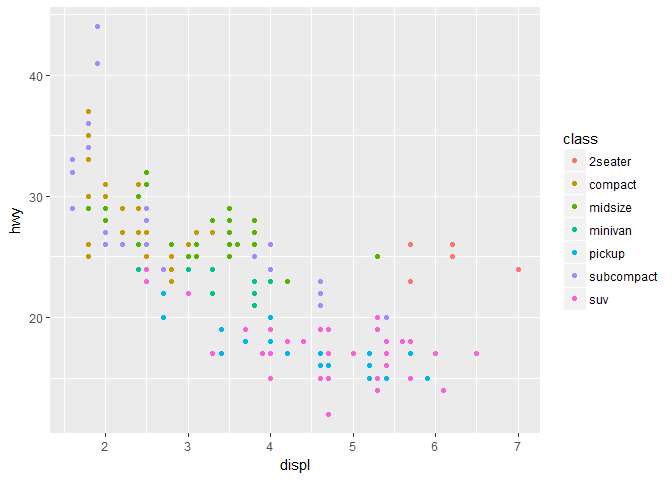
\includegraphics{Class_7_files/figure-latex/unnamed-chunk-54-1.pdf}


\end{document}
